\section{A PIRNN (Physics-Informed Recurrent Neural Network)}

\begin{frame}{Introdução}
  \textbf{PIRNNs} incorporam memória recorrente e permitem uma modelagem mais precisa de sistemas dinâmicos \parencite{zheng_2023}.
  \\ \vspace{0.4cm}
  \begin{figure}
    \centering
    \begin{tikzpicture}[item/.style={circle,draw,thick,align=center},
    itemc/.style={item,on chain,join}]
  \begin{scope}[start chain=going right,nodes=itemc,every
    join/.style={-latex,very thick},local bounding box=chain]
    \path node (A0) {$A$} node (A1) {$A$} node (A2) {$A$} node[xshift=2em] (At)
    {$A$};
  \end{scope}
  \node[left=1em of chain,scale=2] (eq) {$=$};
  \node[left=2em of eq,item] (AL) {$A$};
  \path (AL.west) ++ (-1em,2em) coordinate (aux);
  \draw[very thick,-latex,rounded corners] (AL.east) -| ++ (1em,2em) -- (aux)
  |- (AL.west);
  \foreach \X in {0,1,2,t}
    {\draw[very thick,-latex] (A\X.north) -- ++ (0,2em)
      node[above,item,fill=gray!10] (h\X) {$\nu_\X$};
      \draw[very thick,latex-] (A\X.south) -- ++ (0,-2em)
      node[below,item,fill=gray!10] (x\X) {$x_\X$};}
  \draw[white,line width=0.8ex] (AL.north) -- ++ (0,1.9em);
  \draw[very thick,-latex] (AL.north) -- ++ (0,2em)
  node[above,item,fill=gray!10] {$\nu_t$};
  \draw[very thick,latex-] (AL.south) -- ++ (0,-2em)
  node[below,item,fill=gray!10] {$x_t$};
  \path (x2) -- (xt) node[midway,scale=2,font=\bfseries] {\dots};
\end{tikzpicture}

    \caption{Representação de uma RNN nas formas \textit{folded} e \textit{unfolded}. Fonte: Adaptado de Stack Exchange (2019)}
  \end{figure}
\end{frame}

\begin{frame}
  \textbf{Redes Neurais Recorrentes (RNNs)} usam o \textit{hidden state} ($\nu_t$) para alimentar o mesmo neurônio com as informações dos passos anteriores. Repetindo o processo até obter o estado oculto final \parencite{pytorch_2024}.
  \[
    \nu_t = \sigma(x_t \cdot W_{i\nu}^T + b_{i\nu} + \nu_{t-1} \cdot W_{\nu\nu}^T + b_{\nu\nu})
  \]
\end{frame}

\begin{frame}{Estrutura da PIRNN utilizada}
  A PIRNN utilizada consiste em 5 camadas, todas com a função de ativação tangente hiperbólica $(\tanh)$, com exceção da saída, que não possui função de ativação:

  \begin{itemize}
    \item Entrada: $\mathbf{X} = [[h_1^{(t-1)}, h_1^{(t)}], [h_2^{(t-1)}, h_2^{(t)}], [q^{(t-1)}, q^{(t)}]]$;
    \item \textcolor{red}{camada RNN: 32 neurônios;}
    \item camada linear 1: 32 neurônios;
    \item camada linear 2: 32 neurônios;
    \item camada linear 3: 32 neurônios;
    \item saída: $\mathbf{y} = [h_1^{(t+1)}, h_2^{(t+1)}]$.
  \end{itemize}

  Totalizando $32+32+32+32+2=130$ neurônios.
\end{frame}

\begin{frame}{A função \textit{loss} utilizada}
  A implementação da função \textit{loss} é um tanto diferente: agora não podemos usar a derivação automática, pois o tempo ($t$) não é uma entrada.

  Aqui, foi utilizada a derivada regressiva de 3 pontos (os 2 pontos fornecidos para a rede e o ponto previsto).

  \begin{equation}
    \mathcal{L} = w_1 \cdot \mathcal{L}_{\text{EDO}} + w_2 \cdot \mathcal{L}_{\text{data}}
  \end{equation}
  onde:
  \begin{itemize}
    \item $w_1, w_2$: pesos para o cálculo da Loss;
    \item $\mathcal{L}_{\text{EDO}}$: erro das equações diferenciais;
    \item $\mathcal{L}_{\text{data}}$: erro dos dados;
    \item $\mathcal{L}$: erro total.
  \end{itemize}
\end{frame}

\begin{frame}{Resultados}
  \begin{figure}
    \centering
    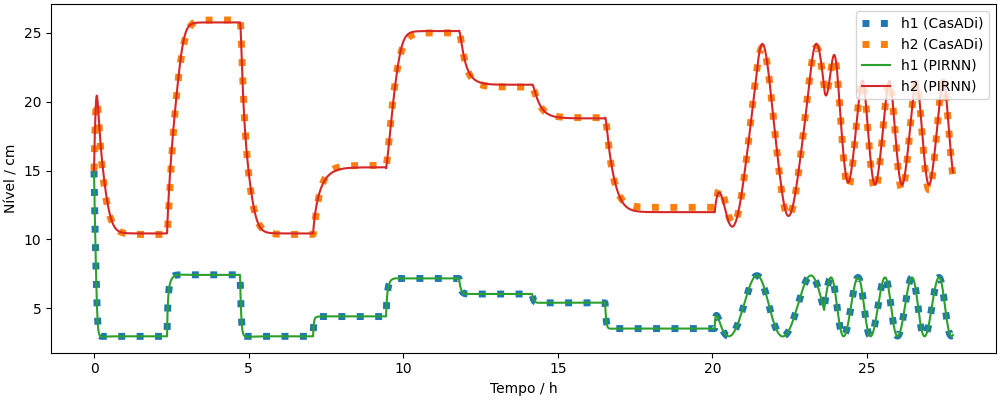
\includegraphics[width=1\textwidth]{pirnn-result.png}
    \caption{Comparação entre as previsões da PIRNN e o método numérico (RK)}
  \end{figure}
\end{frame}

\begin{frame}{Comparação de Tempos de Execução}
  \begin{figure}
    \centering
    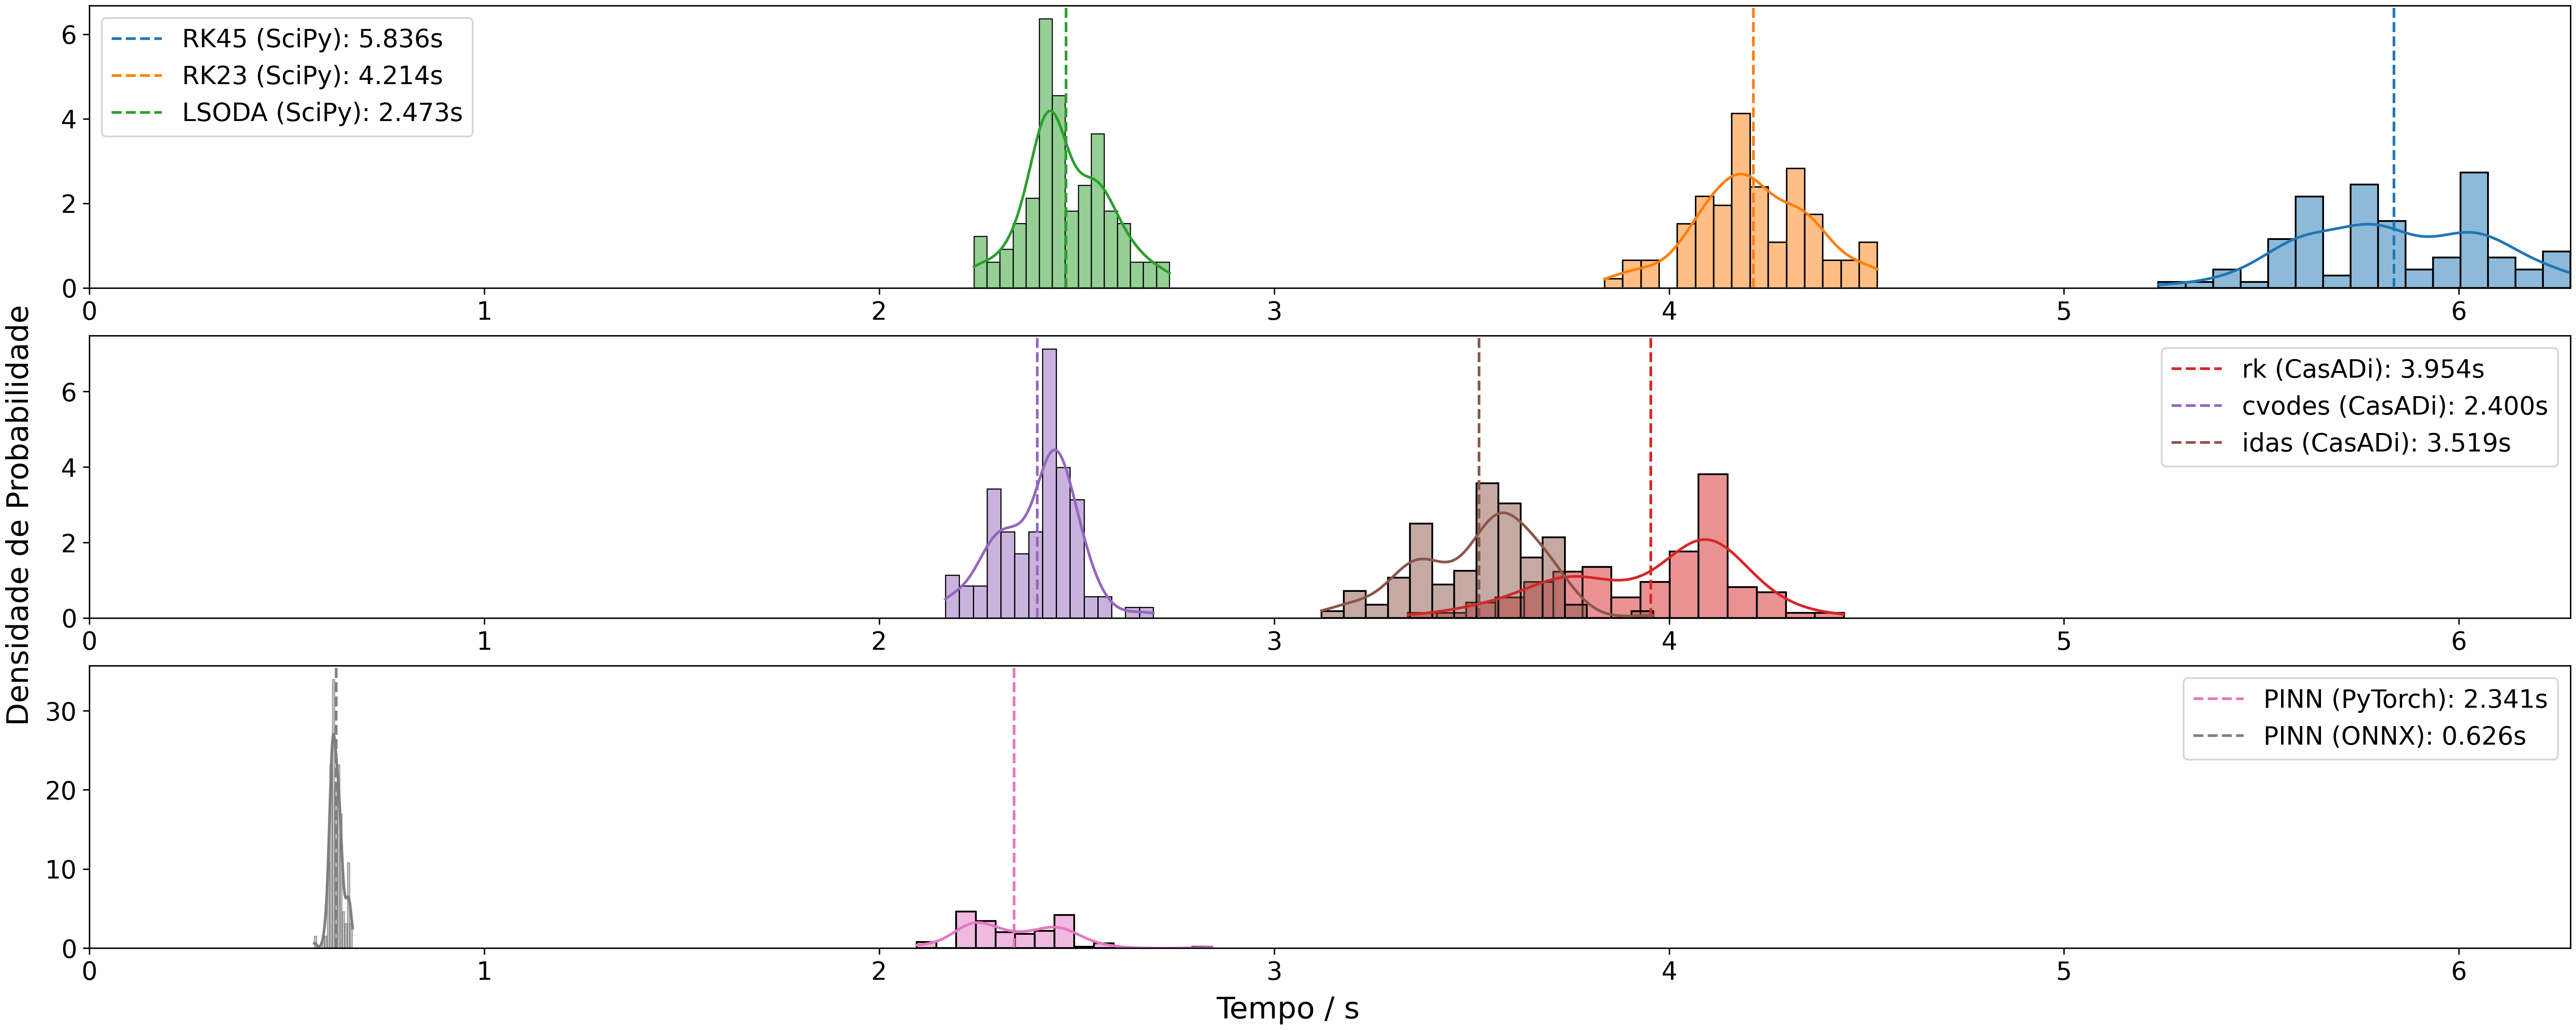
\includegraphics[width=\textwidth]{pirnn-benchmark.png}
    \caption{Densidade de probabilidade dos tempos de execução dos métodos avaliados. Cada método foi executado 100 vezes; as linhas tracejadas indicam os tempos médios.}
  \end{figure}
\end{frame}

\begin{frame}{Por que o ONNX Runtime é tão rápido?}
  \begin{columns}
    \begin{column}{0.5\textwidth}
      O ONNX Runtime é focado em desempenho de inferência e possui uma série de otimizações:
      \begin{itemize}
        \item ``constant folding'';
        \item ``redundant node eliminations'';
        \item ``node fusions''.
      \end{itemize}
    \end{column}
    \begin{column}{0.5\textwidth}
      \begin{figure}
        \centering
        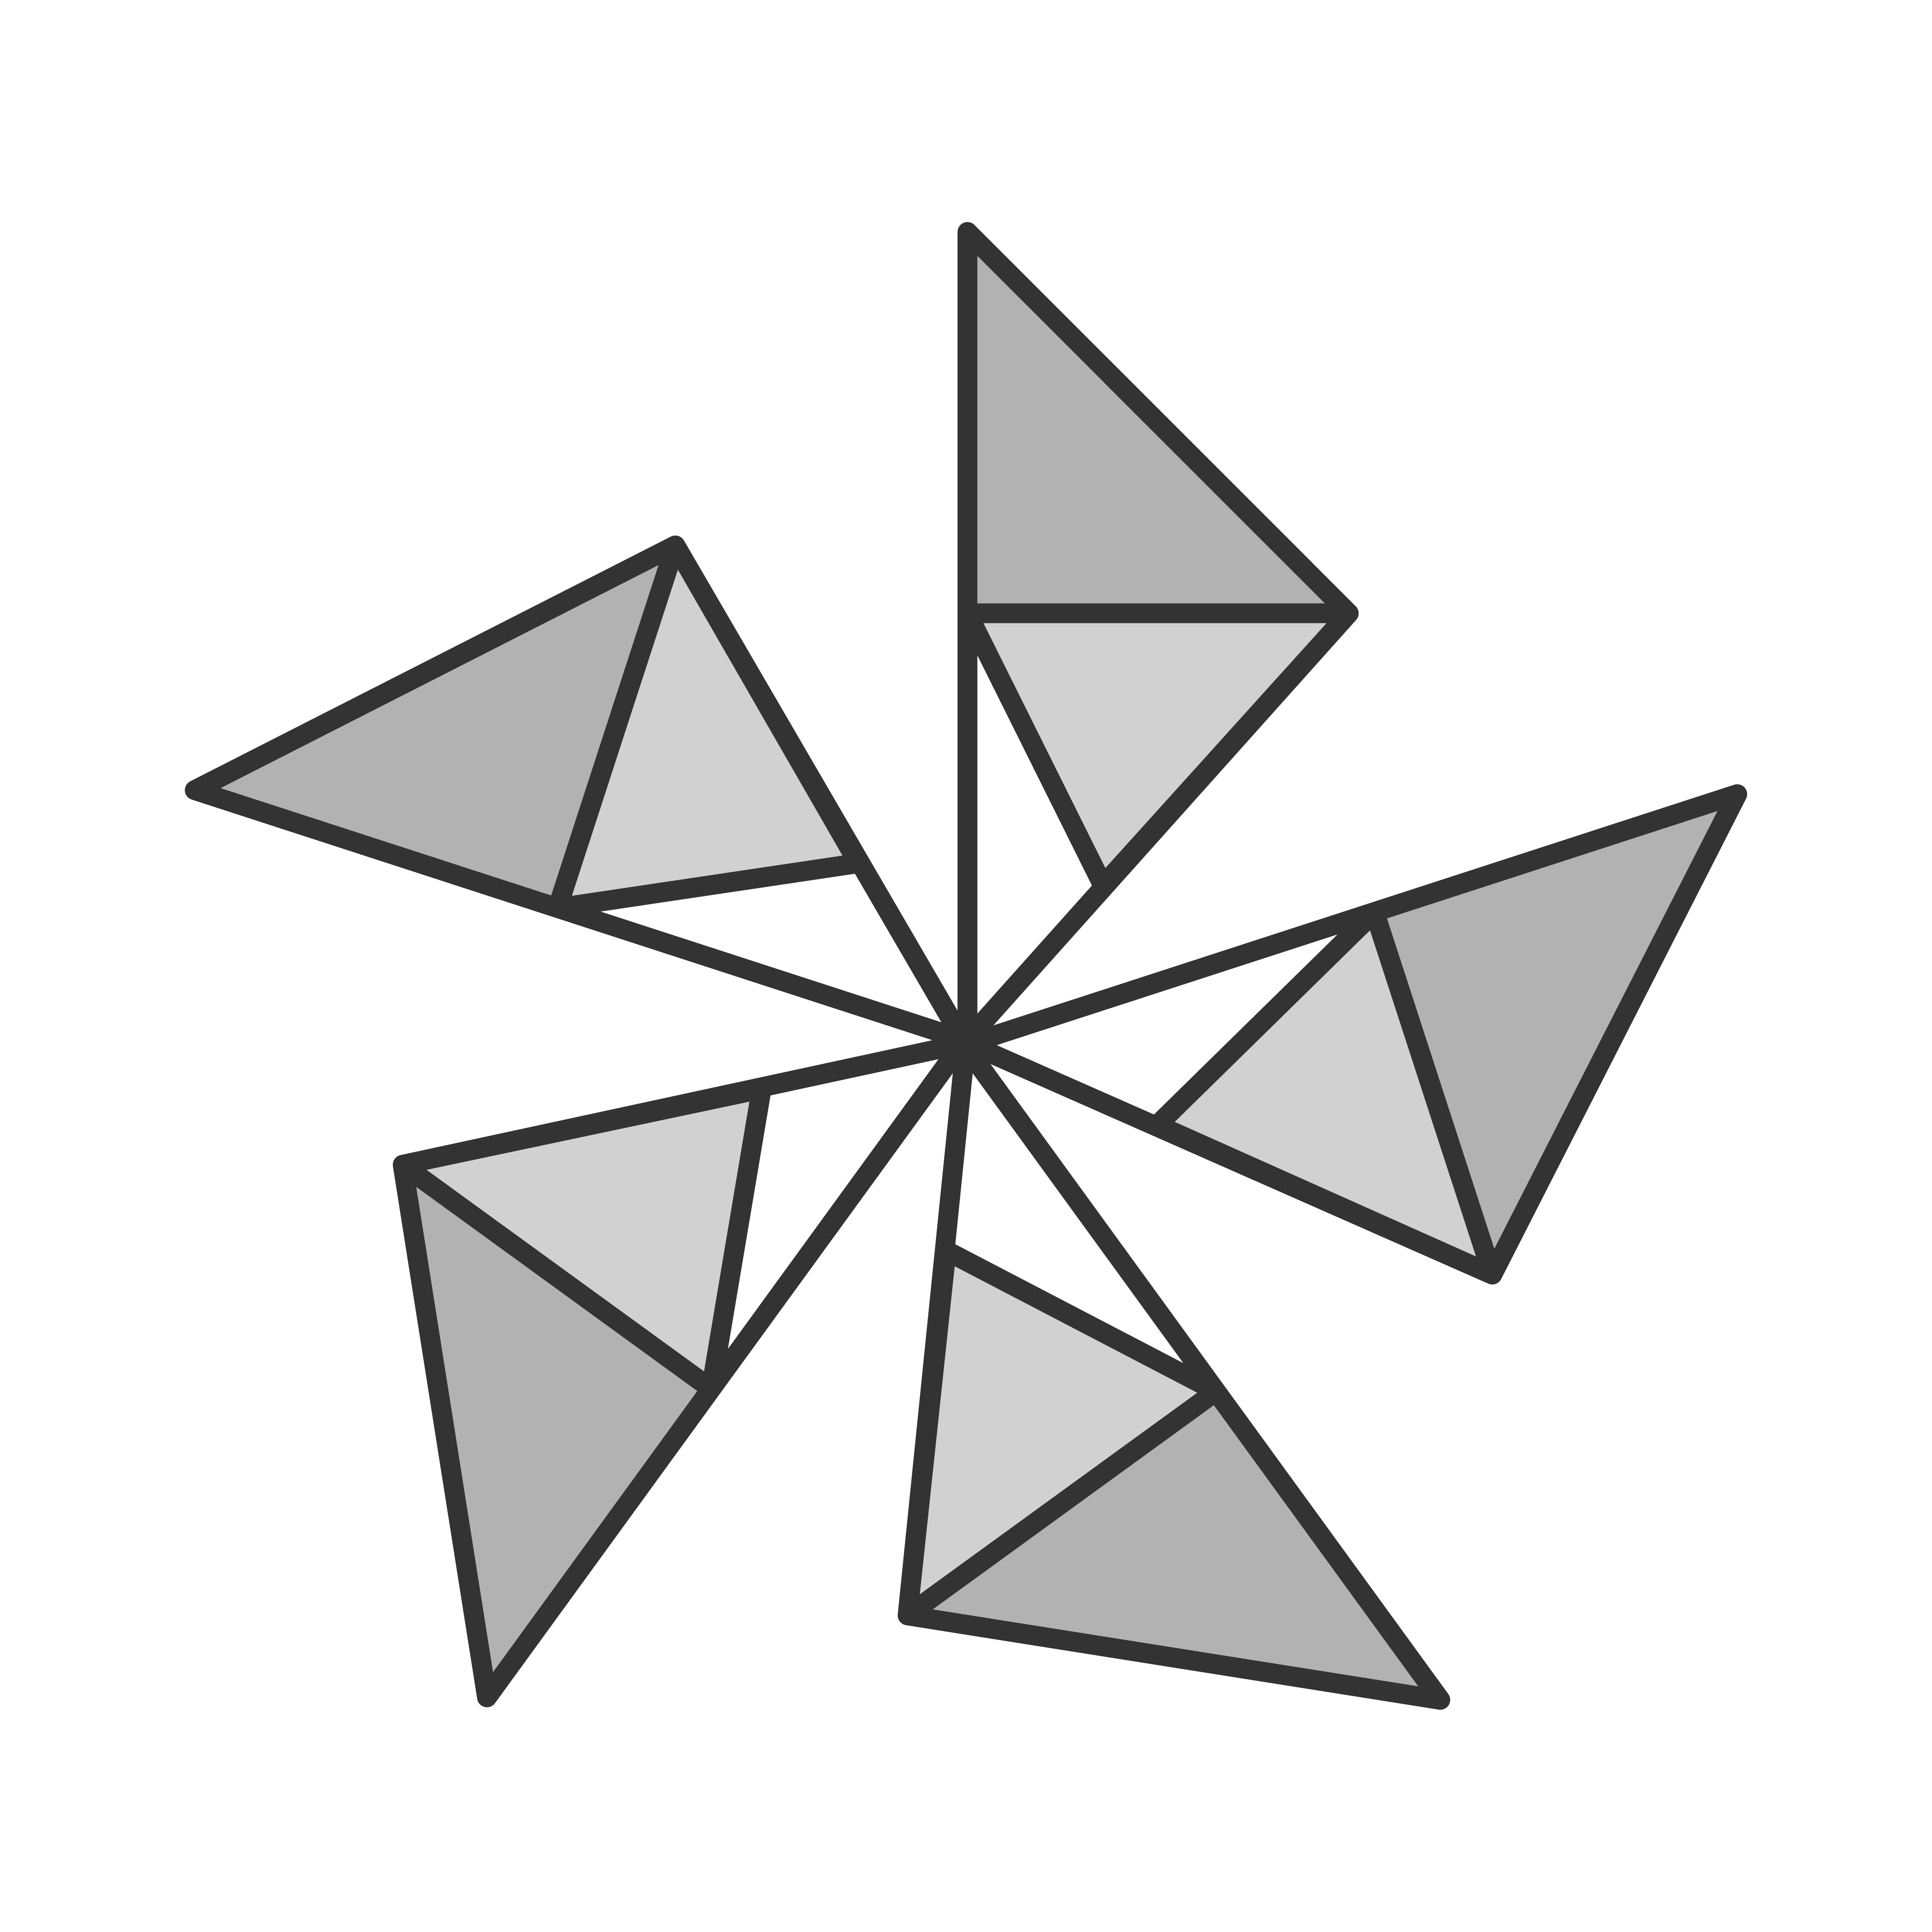
\includegraphics[width=4cm, keepaspectratio]{onnx.png}
        \caption{Logo do ONNX Runtime. Fonte: onnxruntime.ai (2017)}
      \end{figure}
    \end{column}
  \end{columns}
\end{frame}